\date{}
\title{}
\date{}
\begin{document}
\begin{frame}
    \titlepage
\end{frame}

\section{routing problem}

\usetikzlibrary{matrix}
\begin{frame}{routing tables}
\begin{tikzpicture}
\matrix[tight matrix,
    nodes={minimum height=.6cm},gT
    column 1/.style={nodes={text width=4.5cm,font=\small\tt}},
    column 2/.style={nodes={text width=2cm,font=\small\tt,alt=<4>{fill=red!10}}},
    column 3/.style={nodes={text width=1cm,font=\small\tt,alt=<3>{fill=red!10}}},
    row 1/.style={nodes={font=\small}},
    label={north:routing table},
    anchor=north west
] (route table v6) {
IP addresses \& gateway \& iface \\
2001:0db8:40:f000:;/44 \& --- \& int1 \\
2001:0db8:40:e000::/44 \& 2001:0db8:40:f000::2 \& int1 \\
2001:0db8:40:d000::/44 \& --- \& int3 \\
3fff:1000:19::/48 \& --- \& ext1 \\
\ldots \& \ldots \& \ldots \\
\normalfont default \& fe80::17 \& ext2 \\
};
\matrix[tight matrix,
    nodes={minimum height=.6cm},gT
    column 1/.style={nodes={text width=4.5cm,font=\small\tt}},
    column 2/.style={nodes={text width=2cm,font=\small\tt,alt=<4>{fill=red!10}}},
    column 3/.style={nodes={text width=1cm,font=\small\tt,alt=<3>{fill=red!10}}},
    row 1/.style={nodes={font=\small}},
    label={north:routing table},
    anchor=north west
] (route table v4) at (route table v6.south west) {
IP addresses \& gateway \& iface \\
192.0.2.0/25 \& --- \& int1 \\
192.0.2.128/26 \& 192.0.2.1 \& int1 \\
192.0.2.192/26 \& 192.0.2.2 \& int1 \\
198.51.100.0/25 \& 192.0.2.1 \& int1 \\
198.51.100.128/25 \& --- \& int2 \\
\ldots \& \ldots \& \ldots \\
\normalfont default \& 203.0.113.1 \& ext \\
};
\end{tikzpicture}
\end{frame}

\begin{frame}{filling routing tables}
    \begin{itemize}
    \item easy part: what networks are you directly connected to
        \begin{itemize}
        \item that range of IP addresses, that interface
        \end{itemize}
    \vspace{.5cm}
    \item harder part: other routers on connected router
    \item need to learn:
        \begin{itemize}
        \item addresses of other router
        \item which networks can be reached through them directly or indirectly
        \end{itemize}
    \item need to choose between multiple ways of reaching networks
    \end{itemize}
\end{frame}


\section{actions on forwarding}

% FIXME: router picture
\begin{frame}<1>[label=forwardProbs]{problems when forwarding}
    \begin{itemize}
    \item \myemph<2>{no entry in routing table}
    \item \myemph<2>{no entry in neighbor table}
        \begin{itemize}
        \item (after attempting ARP, or neighbor discovery)
        \end{itemize}
    \item \myemph<3>{packet too big for next network}
    \item \myemph<4>{there's an infinite loop in the route}
    \end{itemize}
\end{frame}


\subsection{unreachable}
\againframe<2>{forwardProbs}
\begin{frame}[fragile]{destination host unreachable}
\begin{Verbatim}[fontsize=\small]
$ ping 128.143.67.254
PING 128.143.67.254 (128.143.67.254) 56(84) bytes of data.
From 128.143.63.1 icmp_seq=1 Destination Host Unreachable
From 128.143.63.1 icmp_seq=6 Destination Host Unreachable
^C
--- 128.143.67.254 ping statistics ---
10 packets transmitted, 0 received, +2 errors, 100% packet loss, time 9146ms
pipe 4
\end{Verbatim}
---
\begin{Verbatim}
$ ping6 2606:8e80:7007:ef1a::1
PING 2606:8e80:7007:ef1a::1(2606:8e80:7007:ef1a::1) 56 data bytes
From 2606:8e80:7007:ef1a:cf1f:3948:b5c1:a522 icmp_seq=1 Destination unreachable: Address unreachable
....
\end{Verbatim}
\end{frame}

\begin{frame}{ICMPv6 destination unreachable messages}
\begin{itemize}
\item IPv6 header with ICMP as next protocol
\item 1 byte type = 1 (destination unreachable)
\item 1 byte code =
    \begin{itemize}
    \item examples: address unreachable, administritatively prohibited
    \end{itemize}
\item most of contents of message causing problem
    \begin{itemize}
    \item only most to avoid exceeding max packet size
    \item should let OS figure out which socket to send error to
    \end{itemize}
\end{itemize}
\end{frame}

\begin{frame}{generating destination unreachable}
    \begin{itemize}
    \item by routers: reached correct network, machine not there
    \item by routers: no route to network at all
    \item by routers: administrator rule prohibits forwarding
    \item by destination host: no program listening to that `port'
    \item \ldots
    \vspace{.5cm}
    \item different code values for all cases
    \item machine can also choose to send nothing back
    \end{itemize}
\end{frame}

\begin{frame}{ICMPv4 destination unrachable}
\begin{itemize}
\item basically same format as ICMPv6, but\ldots
\item different type/code integer values
\item only IPv4 header + 64 bytes of original packet included
\end{itemize}
\end{frame}
 % FIXME: wireshark example

\subsection{fragmentation, MTUs}

\againframe<3>{forwardProbs}
\begin{frame}[fragile]{fragmentation}
\begin{itemize}
\item max frame data size on my local network = 1500 bytes, but\ldots
\end{itemize}
\begin{Verbatim}[fontsize=\small]
$ ping6 fe80::da07:b6ff:fed9:ae50 -s 4000
PING fe80::da07:b6ff:fed9:ae50 (fe80::da07:b6ff:fed9:ae50) 4000 data bytes
4008 bytes from fe80::da07:b6ff:fed9:ae50%eno1: icmp_seq=1 ttl=64 time=1.17 ms
4008 bytes from fe80::da07:b6ff:fed9:ae50%eno1: icmp_seq=2 ttl=64 time=0.779 ms
4008 bytes from fe80::da07:b6ff:fed9:ae50%eno1: icmp_seq=3 ttl=64 time=0.742 ms
...
$ ping -s 4000 192.168.1.1                 
PING 192.168.1.1 (192.168.1.1) 4000(4028) bytes of data.     
4008 bytes from 192.168.1.1: icmp_seq=1 ttl=64 time=0.891 ms 
4008 bytes from 192.168.1.1: icmp_seq=2 ttl=64 time=0.806 ms 
4008 bytes from 192.168.1.1: icmp_seq=3 ttl=64 time=0.748 ms 
\end{Verbatim}
\end{frame}

\begin{frame}{fragmentation}
    \begin{itemize}
    \item original sender or router splits packet into multiple
    \item each part called a \textit{fragment}
    \vspace{.5cm}
    \item stored temporarily and ``reassembled'' at receiver
        \begin{itemize}
        \item Linux defaults: \\
        max 64 packet gap between fragments per source IP \\
        30 second time limit before discaded \\
        3-4MB buffer of packets 
        \end{itemize}
    \end{itemize}
\end{frame}

\begin{frame}{IPv6 fragments}
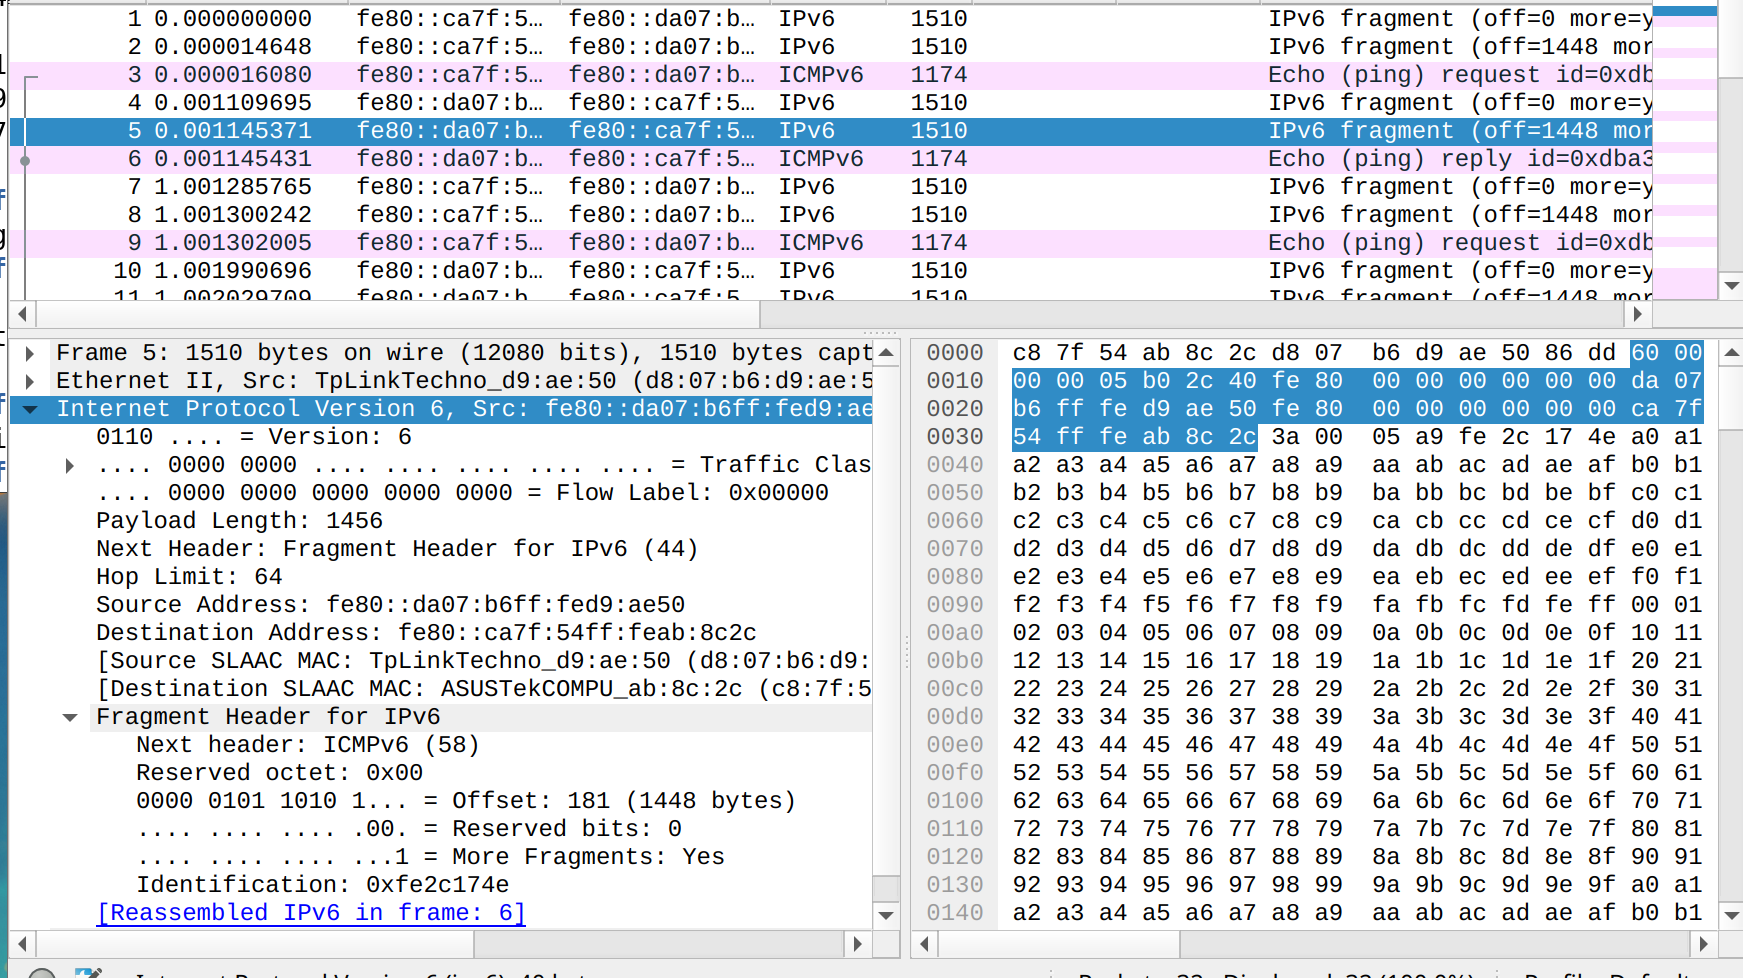
\includegraphics[width=\textwidth]{../routing/ipv6-fragment-ex}
\end{frame}

\begin{frame}{IPv4 fragments}
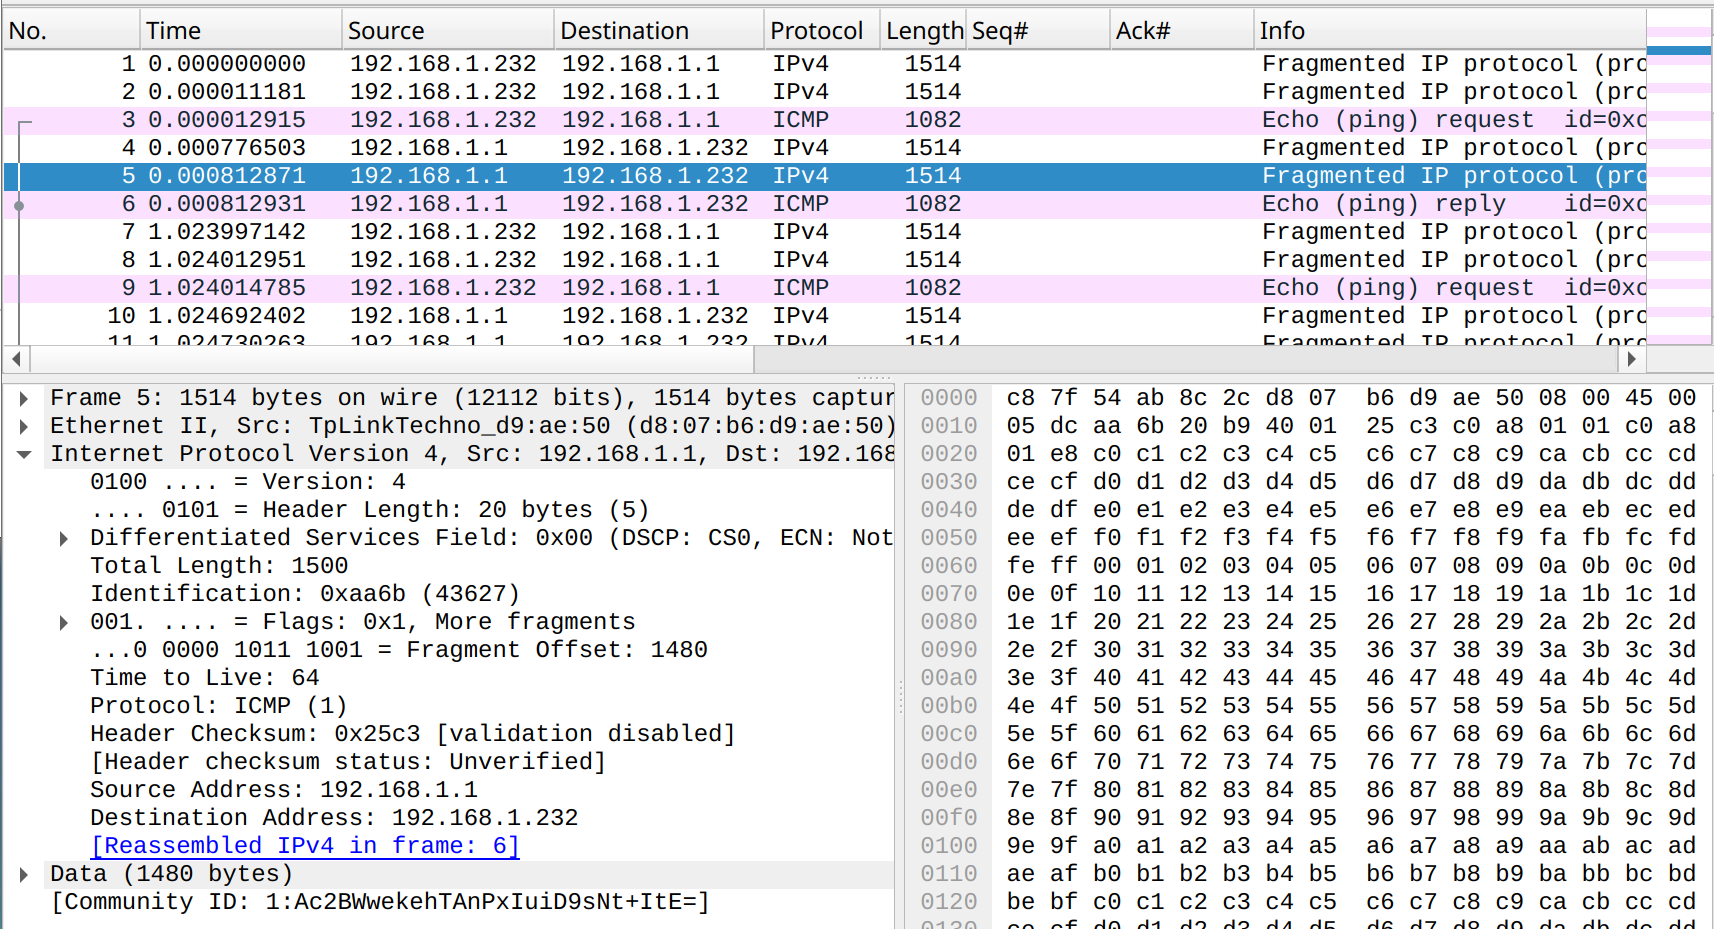
\includegraphics[width=\textwidth]{../routing/ipv4-fragment-ex}
\end{frame}

\begin{frame}{varying frame size support}
    \begin{itemize}
    \item also called \textit{maximum transmission unit} (MTU)
    \vspace{.5cm}
    \item typical Ethernet, Wifi --- 1500 bytes
    \item Ethernet with ``jumbo frames'' -- 65535 bytes
    \item IPsec ESP VPN over 1500-byte MTU network -- $\sim$1400--1440 bytes
        \begin{itemize}
        \item VPN --- simulated network link over other network links
        \end{itemize}
    \end{itemize}
\end{frame}

\begin{frame}{routers making fragments}
    \begin{itemize}
    \item option in IPv4 to handle frame size mismatch, but not great:
    \vspace{.5cm}
    \item extra data sent over network (especially if just over max size)
        \begin{itemize}
        \item extra copies of main headers on each fragment
        \end{itemize}
    \item extra work at receiver to reconstruct fragments
    \item lose whole packet if one fragment is lost
        \begin{itemize}
        \item but other routers likely to still waste time forwarding all other fragments
        \end{itemize}
    \end{itemize}
\end{frame}

\begin{frame}{avoiding fragmentation}
    \begin{itemize}
    \item IPv4 --- DF (don't fragment) flag in packets
        \begin{itemize}
        \item if set, routers not allowed to fragment packet
        \end{itemize}
    \item IPv6 --- routers never fragment packets
        \begin{itemize}
        \item any fragments made at source machine only
        \end{itemize}
    \vspace{.5cm}
    \item<2-> when set --- ICMP error
        \begin{itemize}
        \item ICMPv6: Packet Too Big
        \item ICMPv4: destination unreachable + reason code of fragmentation needed
        \item (hopefully, bad networks might drop packet instead)
        \end{itemize}
    \item<2-> ICMPv6 error tells you maximum supported size
        \begin{itemize}
        \item (by first link that got packet rejected --- might be more constraining link later)
        \item info not available in IPv4
        \end{itemize}
    \end{itemize}
\end{frame}
 % FIXME: IP packet format

\subsection{time-to-live}

\againframe<4>{forwardProbs}
\begin{frame}{time-to-live (v4) / hop limit (v6)}
    \begin{itemize}
    \item stored in IP header 
    \vspace{.5cm}
    \item when forwarding packet, router will:
    \item subtract one from TTL / hop limit
        \begin{itemize}
        \item and recompute checksum accordingly
        \end{itemize}
    \item if TTL/hop limit = 0, drop packet
    \item usually send back ICMP ``Time Exceeded'' error
    \end{itemize}
\end{frame}



\section{traceroute}

\begin{frame}{traceroute}
    \begin{itemize}
    \item ICMP Time Exceeded messages come from router
    \item $\rightarrow$ tells you which routers are involved
    \vspace{.5cm}
    \item<2-> \texttt{traceroute} command: deliberately packets with low TTL/hop limit
    \item<2-> print out what time exceeded messages we get back
    \item<2-> typically sent with TTL/hop limit = 255 so it doesn't get lost
        \begin{itemize}
        \item (`backwards' path might be longer than forwards one)
        \end{itemize}
    \end{itemize}
\end{frame}

\begin{frame}[fragile]{traceroute example}
\begin{Verbatim}[fontsize=\fontsize{8}{9}\selectfont]
traceroute to ripe.net (193.0.11.51), 30 hops max, 60 byte packets
 1  128.143.63.1 (128.143.63.1)  6.367 ms  8.562 ms  8.577 ms
 2  cr01-gil-ae15-00.net.virginia.edu (128.143.221.17)  0.370 ms  0.334 ms  0.349 ms
 3  * * *
 4  br01-udc-et-1-2-0.net.virginia.edu (128.143.236.5)  0.502 ms  0.468 ms  0.488 ms
 5  i2-vt.net.virginia.edu (192.35.48.34)  3.374 ms  3.448 ms  3.413 ms
 6  192.122.175.15 (192.122.175.15)  5.715 ms  5.628 ms  5.590 ms
 7  fourhundredge-0-0-0-17.4079.core1.ashb.net.internet2.edu (163.253.1.8)  29.163 ms
    fourhundredge-0-0-0-16.4079.core1.ashb.net.internet2.edu (163.253.1.2)  28.880 ms
    fourhundredge-0-0-0-17.4079.core1.ashb.net.internet2.edu (163.253.1.8)  28.876 ms
 8  fourhundredge-0-0-0-1.4079.core1.clev.net.internet2.edu (163.253.1.123)  29.568 ms 
    28.667 ms  28.666 ms
 9  fourhundredge-0-0-0-0.4079.core2.newy32aoa.net.internet2.edu (163.253.1.239)  29.608 ms 
    29.476 ms  29.400 ms
10  fourhundredge-0-0-0-19.4079.core1.newy32aoa.net.internet2.edu (163.253.1.40)  28.958 ms 
    28.999 ms 
    fourhundredge-0-0-0-21.4079.core1.newy32aoa.net.internet2.edu (163.253.1.44)  29.280 ms
11  e1-3-2-502.asd001b-jnx-06.surf.net (145.145.166.18)  115.822 ms  115.823 ms  115.744 ms
12  lo0-2.asd001b-jnx-01-surfinternet.surf.net (145.145.128.4)  115.988 ms  115.932 ms  115.918 ms
13  gw.amsix.telrtr.ripe.net (80.249.208.71)  121.956 ms  121.968 ms  121.844 ms
14  * * *
15  * * *
\end{Verbatim}
\end{frame}

\begin{frame}{traceroute sent}
% FIXME: screenshot
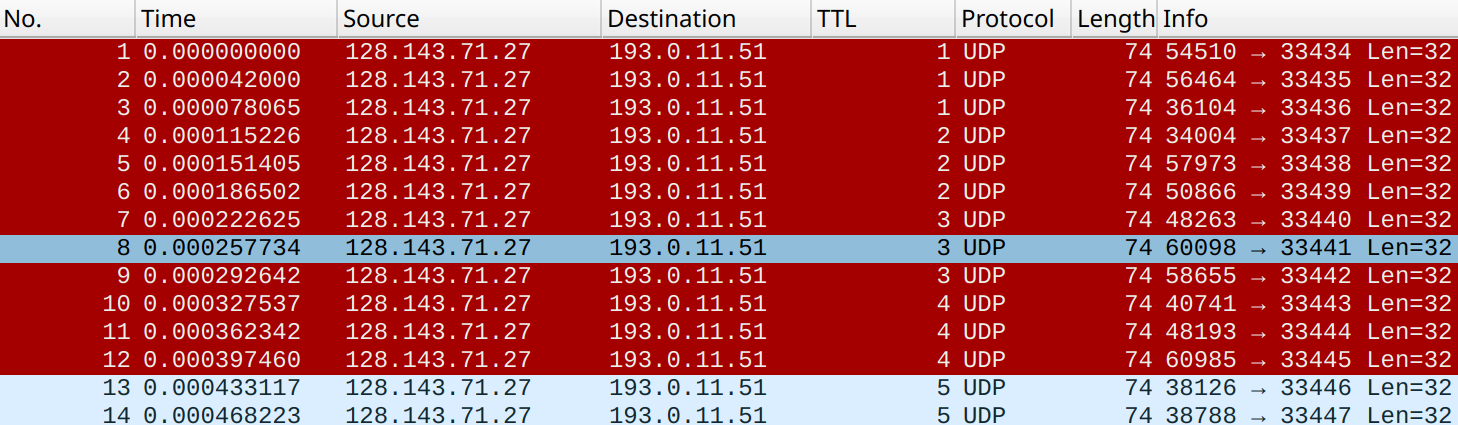
\includegraphics[width=\textwidth]{../routing/traceroute-v4-send}
\end{frame}

\begin{frame}{traceroute received}
% FIXME: screenshot
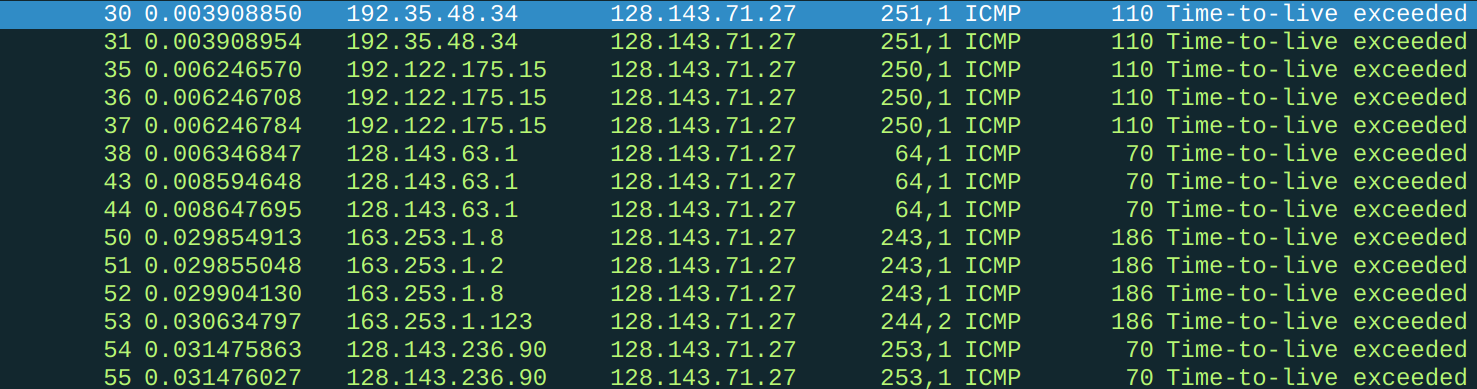
\includegraphics[width=\textwidth]{../routing/traceroute-v4-recv}
\end{frame}

\begin{frame}{aside: multiple paths}
    \begin{itemize}
    \item only showing \textit{forward} path
        \begin{itemize}
        \item routing in reverse direction is often different
        \end{itemize}
    \item sometimes multiple forward paths
        \begin{itemize}
        \item way we've shown routing table so far does not allow this
        \end{itemize}
    \end{itemize}
\end{frame}


\section{centralized versus distributed}
\begin{frame}{constructing routing/neighbor tables}
    \begin{itemize}
    \item interesting task: how to fill tables
    \item two general strategies:
    \vspace{.5cm}
    \item routers/switches learn from neighbors
        \begin{itemize}
        \item ``distributed''
        \end{itemize}
    \item information gathered on single controller machine \\
        which configures routers/switches
        \begin{itemize}
        \item ``centralized''
        \end{itemize}
    \end{itemize}
\end{frame}


\section{basic flooding / MAC learning}
% FIXME

\section{spanning trees}

\subsection{living without TTLs}

\subsection{Union-Find spanning tree}

\subsection{spanning tree protocol}

\section{aside: metrics}

\section{Bellman-Ford}

\section{distance vector routing}

\subsection{centralized algorithm}

\subsection{distributed algorithm}

\section{link state}

\section{interdomain routing}

\subsection{business priorities}

\subsection{sharing routes: BGP}

\subsection{loop prevention, metrics}

\subsection{within-AS routing}

\subsection{hot or cold potato}

\section{backup slides}
\begin{frame}{backup slides}
\end{frame}

\end{document}
